\documentclass{article}
\usepackage[utf8]{inputenc}
\usepackage[margin=3cm]{geometry}
\usepackage{indentfirst}
\usepackage{graphicx}
\graphicspath{ {./images/} }
\setlength{\parindent}{0.75cm} %heh, 0.75

\title{
    \textbf{Programação 3D - Assignment I}
    }
\author{
    \begin{Large}
        \textbf{Grupo 02}
    \end{Large}\\
    Francisco Campaniço 83463\\
    João Rafael 83482\\
    Rodrigo Oliveira 83558
}
\date{Março 2019}

\begin{document}

    \maketitle

    \section*{\textit{Parser} NFF}

        \par 
        O programa começa por ler o ficheiro NFF definido pelo utilizador no início do código. Seguindo a especificação do formato NFF, adiciona uma câmara, luzes e objetos à cena. A cena (classe \texttt{Scene}) contêm uma câmara, um número de luzes definido pelo ficheiro NFF, e objetos também definidos pelo mesmo.
        \par
        Um objeto (classe \texttt{SceneObject}) contém uma classe \texttt{Material} e métodos genéricos de interseção e cálculo de normais, que são \textit{overriden} pelas classes que herdam desta.
        \par
        Dado que o formato NFF não têm uma opção para \textit{Bounding Boxes}, foi adicionada uma opção para tal: \texttt{aabb x0 x1 y1 y2 z1 z2}, que cria uma AABB com os limites em cada eixo declarados pelas variáveis seguintes.

    \section*{Interseções}

        \par
        O raio verifica interseções com objetos ao chamar o método \texttt{intersect} de cada objeto, que devolve um \textit{boolean} e a distância \textit{t} da origem do raio ao objeto. Depois disto, o objeto com menor \textit{t} é o mais próximo, logo os cálculos seguintes de iluminação aplicam-se a este.

        \par
        A tabela abaixo contém os resultados de tempo para cada um dos testes disponibilizados. Estes resultados foram obtidos num portátil com um CPU Intel Core i7-8750H (6 \textit{cores}, 2.2GHz) e uma GPU NVIDIA GeForce GTX 1060, correndo Kubuntu 18.04 e usando o programa Unix \texttt{time} para determinar o tempo de execução.

        \begin{table}[h]
            \centering
            \begin{tabular}{|l|l|l|l|l|}
                \hline
                Teste & Low     & Medium    & High     & Very High \\ \hline
                Balls & 0m11s   & 0m18s     & 12m14s   & -         \\ \hline
                Mount & 0m15s   & -         & 8m58s    &           \\ \hline
            \end{tabular}
        \end{table}
    \subsection*{Raio-Esfera}

        \centering
        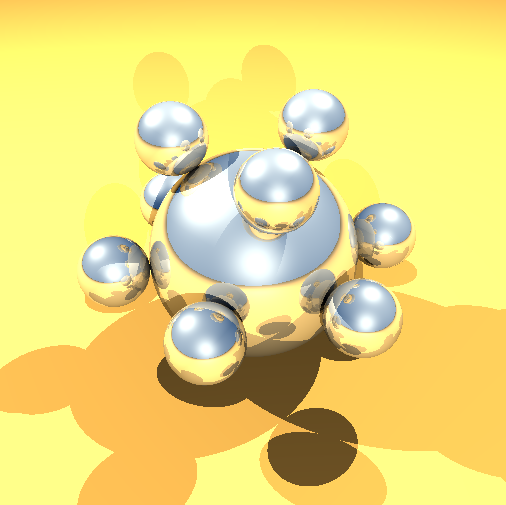
\includegraphics[scale=0.27]{deez_low}
        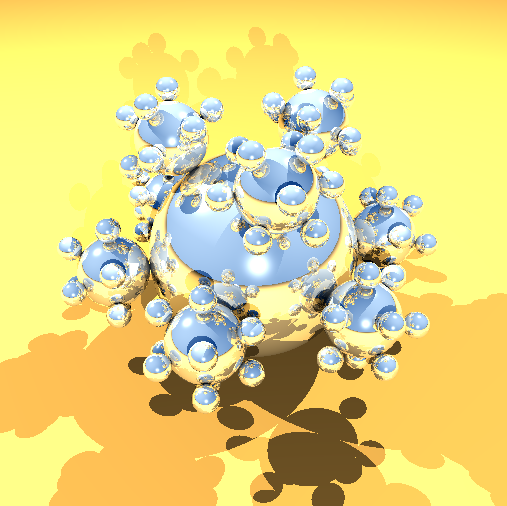
\includegraphics[scale=0.27]{deez_med} 
        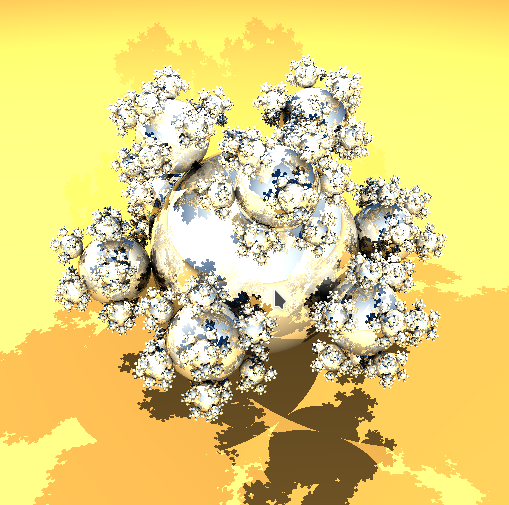
\includegraphics[scale=0.27]{deez_high} 

    \subsection*{Raio-Plano}

    \subsection*{Raio-Triângulo}

        \par
        Para calcular a interseção entre raios e triânglos, utiliza-se o algoritmo de Möller-Trumbone.

        \centering
        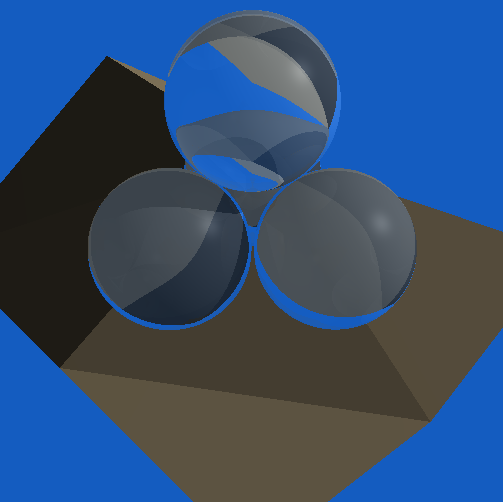
\includegraphics[scale=0.27]{mount_low}
        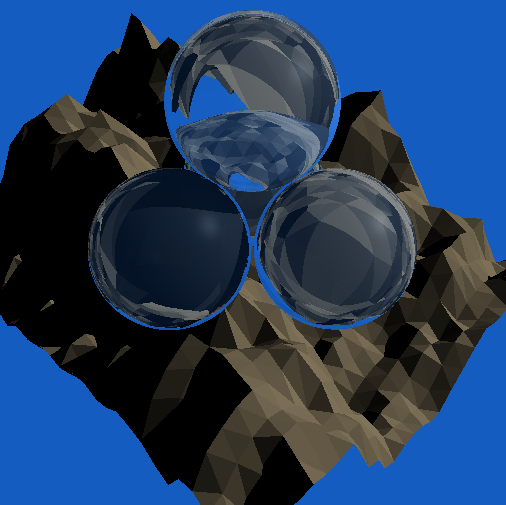
\includegraphics[scale=0.27]{mount_med} 
        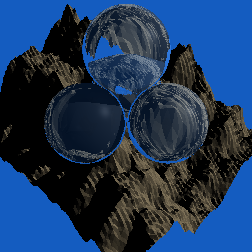
\includegraphics[scale=0.27]{mount_high} 

    \subsection*{Raio-Cone (Extra)}

    \subsection*{Raio-AABB (Extra)}

    \section*{Iluminação Blinn-Phong}

    \section*{Sombras}

    \section*{Reflexão}

    \section*{Refração}

\end{document}